\chapter{Discipline and Procrastination}

This lecture comes to us as a Jim Rohn talk from a curated LazyingArt LLC playlist, and its formal structure is verbal rather than blackboard-based. Still, the opening is unusually sharp. We are not asked to admire discipline from a distance; we are asked to see it as a precise relation between awareness and action. From there the lecture unfolds almost like a small dynamical system: awareness may pass straight into implementation, or it may be delayed; reward may be delayed and large, or immediate and small; discipline may spread through the whole life, or laziness may do the same. These notes keep that order and make the underlying structure explicit where the transcript supports it.

\section{Discipline and Procrastination as a Time Relation}

We begin exactly where the lecture begins. Discipline is not first presented as personality, mood, or moral decoration. It is presented as a pairing: the awareness that action is needed, and the conscious act of carrying that action out.

\begin{equation}
D := (\text{awareness of the need for action}) + (\text{conscious implementation of that action}).
\end{equation}

If we want a compact notation for the lecture's first distinction, we may introduce a time lag between the moment of awareness and the moment of implementation:
\begin{equation}
\Delta t := t_{\mathrm{impl}} - t_{\mathrm{aware}}.
\end{equation}
This notation is editorial, but it catches the exact force of the opening. The lecture says that when awareness and implementation occur together, a valuable sequence of disciplined activity begins; when a considerable time passes between them, we have procrastination. In the simplest cleaned-up form,
\begin{align}
\Delta t \approx 0 &\Rightarrow \text{disciplined activity}, \\
\Delta t \gg 0 &\Rightarrow \text{procrastination}.
\end{align}

\begin{figure}
\centering
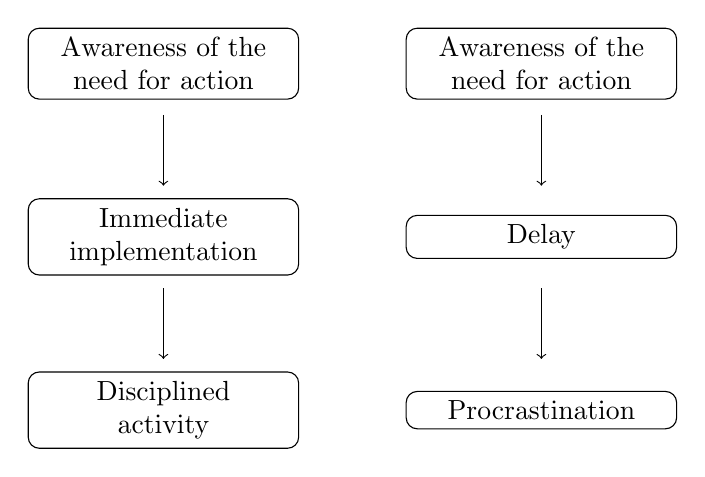
\begin{tikzpicture}[x=1cm,y=1cm]
\node[draw, rounded corners, align=center, text width=3.2cm] at (-2.4,0) {Awareness of the\\need for action};
\node[draw, rounded corners, align=center, text width=3.2cm] at (-2.4,-2.2) {Immediate\\implementation};
\node[draw, rounded corners, align=center, text width=3.2cm] at (-2.4,-4.4) {Disciplined\\activity};

\node[draw, rounded corners, align=center, text width=3.2cm] at (2.4,0) {Awareness of the\\need for action};
\node[draw, rounded corners, align=center, text width=3.2cm] at (2.4,-2.2) {Delay};
\node[draw, rounded corners, align=center, text width=3.2cm] at (2.4,-4.4) {Procrastination};

\draw[->] (-2.4,-0.65) -- (-2.4,-1.55);
\draw[->] (-2.4,-2.85) -- (-2.4,-3.75);
\draw[->] (2.4,-0.65) -- (2.4,-1.55);
\draw[->] (2.4,-2.85) -- (2.4,-3.75);
\end{tikzpicture}
\end{figure}

What the lecture does next is important. It does not leave the distinction in technical language. It compresses it into speech we can carry around: the voice of discipline says, do it now. The voice of procrastination says, later, tomorrow, whenever I get a chance. That compression is not a simplification away from the structure; it is the structure translated into ordinary speech.

\subsection{Question \& Answer}

Question. What exactly separates discipline from procrastination?

Answer. Not knowledge alone, and not desire alone. The lecture's answer is that the crucial difference lies in the interval between awareness and implementation. We may know what must be done in both cases. The difference is whether action follows at once, or whether it is pushed away.

\paragraph{Worked comparison.}
We can summarize the opening logic in four steps.
\begin{enumerate}
\item We become aware that an action is needed.
\item We either implement that action or postpone it.
\item If implementation follows awareness directly, a disciplined sequence begins.
\item If implementation is delayed substantially, the same situation is renamed procrastination.
\end{enumerate}

\section{Do It Now or Do It Later: Fruit and Reward Timing}

Once the opening distinction is in place, the lecture widens it. The point is no longer merely that one pattern is prompt and the other delayed; the point is that each pattern grows into a kind of life. The lecture says that discipline bears the fruit of achievement and contentment, while procrastination bears no fruit, only the bare branches of mediocrity. One line in this region is garbled, but that image is clear, and it is worth preserving.

The whole contrast is then reduced again to a pair of slogans:
\begin{equation}
\text{discipline} \leftrightarrow \text{do it now}, \qquad
\text{procrastination} \leftrightarrow \text{do it later}.
\end{equation}
The slogans matter because they allow the lecturer to move from time relation to reward structure. The rewards of discipline are great, but they are delayed; the rewards of indiscipline are immediate, but they are minor.
\begin{equation}
\text{rewards of discipline} = \text{great but delayed}, \qquad
\text{rewards of lack of discipline} = \text{immediate but minor}.
\end{equation}

The beach example is the lecture's way of making this asymmetry concrete:
\begin{equation}
\text{immediate reward of indiscipline} = \text{a fun day at the beach}, \qquad
\text{future reward of discipline} = \text{owning the beach}.
\end{equation}
That is a compact business morality. The lecture is not doing economics here; it is clarifying why the wrong choice remains attractive. The smaller reward arrives sooner. The larger reward asks for patience, repetition, and the ability to endure the interval.

A useful shorthand, again editorial but faithful, is
\begin{equation}
\text{today's pleasure} > \text{tomorrow's fortune}
\end{equation}
as a description of what people commonly choose. The sign is not a moral endorsement. It only records the fact that most of us often rank the near reward above the distant one.

\subsection{Question \& Answer}

Question. If indiscipline feels rewarding now, why is it not the better bargain?

Answer. Because the lecture's comparison is not between reward and no reward, but between two different reward schedules. One pays quickly and poorly. The other pays slowly and richly. The temptation of procrastination is real precisely because it is not empty; it is simply small, immediate, and strategically disastrous.

\section{Distraction, Focus, and the Power of Association}

Once the lecture has exposed the reward asymmetry, it turns practical. We get a rapid run of questions: how do we get rid of easy distractions? How do we keep the mind on the work? How do we choose discipline over procrastination? How do we avoid the water cooler? The lecture wants us to feel that this is now the active problem, not a philosophical puzzle.

The answer begins plainly: keep the focus on the work, get it done today instead of tomorrow, and work on consistent self-discipline daily. The interesting move is that distraction is not treated as a single thing. It is broken into a small list of sources:
\begin{equation}
(\text{negative thoughts},\ \text{negative people},\ \text{water-cooler chatter},\ \text{doubts within oneself}).
\end{equation}
So the problem of discipline becomes ecological. We are not merely managing an inner will. We are also managing associations, conversations, atmospheres, and habits of attention.

The lecturer is especially sharp about association. Depending on the type of people with whom we associate, we will be distracted. That is an important transition, because it broadens discipline from a private virtue into a boundary condition on the life we inhabit. The distractions of the room become the distractions of the mind, and the distractions of the mind become postponed action.

\subsection{Question \& Answer}

Question. How do distractions and associations actually defeat disciplined action?

Answer. They widen the distance between awareness and implementation. The work is still known, but it is pushed aside by chatter, mood, social gravity, and inward uncertainty. That is why the lecture insists on daily consistent self-discipline: the issue is not one heroic decision, but the repeated closing of the gap.

\section{First Step: Discipline Is Not the Easiest Option}

At this point the lecture organizes itself explicitly. We are told that there are three steps to becoming disciplined, and the first is realism: true discipline is not the easiest option.
\begin{equation}
\text{true discipline} \neq \text{the easiest option}.
\end{equation}
This is not merely a slogan. The lecturer unpacks it through examples: sleeping late is easier than rising early, watching television is easier than opening a book, waiting is easier than acting, trying is easier than doing.

The examples matter because they show that difficulty is not accidental to discipline. It belongs to the phenomenon. Discipline, in the lecture's sense, is already a refusal to let ease govern the ranking of actions. That is why the rhetorical question arrives exactly here: what would become of us if we did not have to make the bed, keep the garage clean, pay taxes, or show up for work? The answer is blunt: not much.

The lecture then turns that observation into a structural claim:
\begin{equation}
\text{the easiest things in life} \Rightarrow \text{the most unprofitable}, \qquad
\text{the profitable} \Rightarrow \text{the most difficult}.
\end{equation}
Again, we should not over-read the word ``profitable.'' This is not finance theory. It is a moral description of how life is arranged. Ease gives momentary reward. Discipline gives significant reward. Thus the world appears as a continual contest:
\begin{equation}
\text{life} = \text{battle between ease with momentary rewards and discipline with significant rewards}.
\end{equation}

The price language comes next and gives the section its formal closure. Each path has a price: the price of discipline or the price of regret. We will pay one or the other. If we want the comparison in the tersest form, we may write
\begin{equation}
\text{price of discipline} < \text{price of regret},
\end{equation}
but this inequality is only editorial shorthand. The lecture's own phrasing is better remembered as a verbal pair: discipline costs pennies, regret costs a fortune.

\subsection{Question \& Answer}

Question. Why is the easiest option usually the least profitable one?

Answer. Because the lecture's world is arranged so that ease brings momentary reward, not substantial return. The easy act spares us the immediate cost; it does not spare us the eventual bill. Regret is therefore not an accidental mood added at the end. It is the accumulated price of preferring ease at each local decision.

\section{Second Step: Discipline as Full-Time Consistency}

The transcript around the middle is damaged in places, but the lecture's next stable move is unmistakable: the best form of discipline is consistent self-discipline.
\begin{equation}
\text{best form of discipline} = \text{consistent self-discipline}.
\end{equation}
The examples are homely and therefore strong. The discipline required to make the bed every day is the same discipline required for business success. The discipline required to organize the garage is the same discipline required to organize the business. The point is not that all tasks are equal. The point is that all disciplines carry through to affect all parts of life.

That principle can be written in a compact pair:
\begin{align}
\text{discipline in one area} &\Rightarrow \text{discipline in larger areas}, \\
\text{lazy side} &\to \text{destroys disciplined side}.
\end{align}
The second line is crucial. The lecture does not merely say that discipline spreads. It says that laziness spreads too. A life cannot safely be part disciplined and part abandoned, because the abandoned region leaks into the ordered one.

This is why the lecturer gives the maxim
\begin{equation}
\text{consistency cannot be inconsistent}.
\end{equation}
The phrase sounds tautological, but it is not empty. It means that consistency is not a local achievement. It is a property of the whole pattern of conduct.

The lecture then deepens the definition:
\begin{equation}
\text{discipline} := \text{the mind being trained to control our lives}.
\end{equation}
This is a stronger formulation than the opening one. At the start, discipline was awareness plus implementation. Here it becomes the shaping of the mind itself so that awareness and implementation will reliably meet.

\subsection{Question \& Answer}

Question. Can discipline remain local to one area while we are lazy in another?

Answer. The lecture says no. The same structure that orders a bed, a garage, or a business also connects those regions. A lazy habit is not content to remain isolated. It creeps. That is why consistent self-discipline must be full-time rather than occasional.

\paragraph{Transfer rule.}
The lecture's practical transfer principle may be read in five short steps.
\begin{enumerate}
\item A small daily discipline is established.
\item That discipline shapes the way we meet ordinary obligations.
\item The same pattern appears in larger tasks and responsibilities.
\item If a lazy region is protected instead, it spreads by the same mechanism.
\item Therefore discipline must be treated as global rather than compartmental.
\end{enumerate}

\section{Standards, Hypocrisy, and the Absence of Discipline}

Once discipline becomes full-time, the lecture moves from habits to standards. We have, it says, standards that we have selected as a personal code of conduct. Let us denote that code by
\begin{equation}
C := \text{a selected personal code of conduct}.
\end{equation}
Discipline then acquires another definition:
\begin{equation}
\text{discipline} := \text{imposing on ourselves the requirements for honoring our standards}.
\end{equation}
This is a valuable tightening. It means that discipline is not merely effort. It is effort under a chosen law.

From here the lecture turns toward hypocrisy. We shout our beliefs, condemn contrary beliefs, instruct children and employees, and yet do not walk the talk. The failure is not merely social embarrassment. It is structural:
\begin{equation}
\text{announced standards} \land \text{unlived conduct} \Rightarrow \text{loss of credibility outwardly and inwardly}.
\end{equation}
The outer loss is obvious. Others stop trusting the standard. The inner loss is more important. We stop trusting ourselves as people who mean what they say.

The lecture then sharpens the negative image. Worse than the inconsistent disciplinarian is the person who has never considered the need or value of discipline at all. Such a person wanders, changes commitments, leaves behind unfinished projects, broken friendships, and unfulfilled promises. The image may be compressed as
\begin{equation}
\text{no sense of the need or value of discipline} \Rightarrow \text{wandering commitments} + \text{broken friendships} + \text{unfinished projects} + \text{unfulfilled promises}.
\end{equation}
Here the lecture widens from productivity into character. We are no longer only asking whether tasks get done. We are asking what sort of trail a life leaves behind.

\subsection{Question \& Answer}

Question. What breaks first when our standards are declared but not lived?

Answer. Credibility breaks first, and it breaks twice. Others lose faith in our words, and we lose faith in our own power to honor the code we have selected. That double break is why the lecture treats inconsistency as more than inefficiency. It is a fracture of the self-government on which discipline depends.

\section{Third Step: Multiple Reward, Boundaries, and Self-Imposed Discipline}

Only after the cost of ease, the need for consistency, and the danger of hypocrisy have been established does the lecture arrive at the third step. That is good sequencing. The promise is allowed to arrive late, after the work of taking discipline seriously has been done.

The third step is a law-like claim:
\begin{equation}
\text{for every disciplined effort, there is a multiple reward}.
\end{equation}
This is one of the lecture's strongest formal lines. It is immediately tied to sowing and reaping:
\begin{equation}
\text{if you sow well, you reap well}, \qquad
\text{we reap what we've sown and we reap much more}.
\end{equation}
The essential point is multiplication. The lecture is not saying that disciplined effort merely returns itself. It says that disciplined effort returns enlarged.

That claim is then generalized through examples. Unique service, fairness, honesty, patience, and giving more than one expects to receive all fall under the same law. The key word remains discipline. The reward multiplies because the disciplined act becomes a seed rather than a single isolated event.

This prepares the final widening. Everything of value requires care and attention; everything of value requires discipline.
\begin{equation}
\text{everything of value requires care and attention}, \qquad
\text{everything of value requires discipline}.
\end{equation}
Children require discipline, because they need structure and boundaries within which to grow. Thoughts require discipline, because without inner boundaries our thinking becomes confused. The lecture's cognitive conclusion is simple and exact:
\begin{equation}
\text{confused thoughts} \Rightarrow \text{confused results}.
\end{equation}

The lecture then turns personal again. The most valuable form of discipline is the one we impose on ourselves:
\begin{equation}
\text{most valuable discipline} = \text{self-imposed discipline}.
\end{equation}
That line matters because it closes the circle. The opening definition described discipline operationally. The ending describes it morally. A person who will not impose order on himself must eventually be ruled from outside, or simply deteriorate into drift.

The final classification of lives is therefore fitting:
\begin{equation}
\text{life} \in \{\text{warning},\ \text{example}\}.
\end{equation}
That is the chapter's closing register. Discipline is no longer merely a technique for getting things done. It is the difference between a life that instructs by failure and a life that instructs by form.

\subsection{Question \& Answer}

Question. Why does self-imposed discipline yield more than it seems to cost?

Answer. Because in the lecture it is not a subtractive act. It is seed-like. It sets in motion a multiplying return: steadier action, stronger credibility, better boundaries, clearer thought, and larger future reward. External discipline may still produce order, but it comes late and carries a tragic implication, namely that someone else cared more for our order than we did.

\paragraph{Boundary principle.}
The lecture applies the same structure in two domains.
\begin{enumerate}
\item Children need boundaries in order to feel secure enough to grow.
\item Thoughts need boundaries in order not to collapse into confusion.
\item In both cases discipline is not suffocation but shape.
\item Therefore discipline is presented not as the enemy of life, but as the condition under which value can develop.
\end{enumerate}

\section{Summary}

The lecture begins with a precise relation and ends with a judgment on whole lives. First, discipline is awareness joined to implementation, while procrastination is the gap between them. Then the talk shows us the two paths in their full consequences: do it now or do it later, fruit or bare branches, delayed large rewards or immediate small ones. From there it moves through distraction, the refusal of ease, the price of regret, the demand for consistency, the honoring of standards, the danger of hypocrisy, and finally the law that disciplined effort multiplies its return.

What makes the lecture hold together is that each later claim can be traced back to the opening relation. If awareness and action are separated, mediocrity begins. If they are joined, discipline begins. The entire talk is an elaboration of that fact. In the end, the lecturer asks us to judge a life not by intention alone but by form: our lives will stand either as warnings or as examples.